

% Nastaven� �ablony FM TUL
% nastaveni prezentace
%\documentclass[draft]{beamer}
\documentclass[t]{beamer}

\usepackage[czech]{babel}

% FONTY

%\usepackage[cp1250]{inputenc} % pro win1250
\usepackage[T1]{fontenc}

\usepackage[utf8]{inputenc}
%\usepackage[IL2]{fontenc}

\usepackage{lmodern}

% XeLaTeX
%\usepackage{fontspec,lipsum}
%\defaultfontfeatures{Ligatures=TeX}
%\usepackage[small,sf,bf]{titlesec}
% 
%\setromanfont{Georgia}
%\setsansfont{Myriad Pro} %Tahoma}
%\setsansfont{Tahoma}
%\setsansfont{Arial}
%\setsansfont{Times New Roman}
%====

% bohu�el dal�� fonty nejsou pln� po�e�t�n�, tedy nejde bez obt��� kop�rovat z PDF

%\usepackage{times}
% \usepackage{avant}
% \usepackage{bookman}
% \usepackage{helvet}  %chyb� tu�n� �ez u strojov�ho p�sma
% \usepackage{newcent}
% \usepackage{palatino} 



%\usepackage[scaled]{uarial}
%\usepackage{helvet}


\usepackage{hyperref}

\mode<presentation>
{
  \definecolor{FM_TUL}{cmyk}{0,0.6,1,0}
  
  \useinnertheme{rectangles}
  
  % VN�J�� BAREVN� T�MA NADPIS�    
  \usecolortheme{whale}  
  
  % VNIT�N� BAREVN� T�MA V��T�, BLOK� ATD.  
  \usecolortheme{orchid}

  \setbeamercolor{titlelike}{parent=structure}
  \setbeamercolor{frametitle}{fg=black}
  \setbeamercolor{title}{fg=black}
  \setbeamercolor{item}{fg=FM_TUL} 
  \setbeamertemplate{navigation symbols}{} % potla�en� naviga�n�ch symbol�
  \setbeamercolor{block title}{fg=white,bg=FM_TUL} % p�edefinov�n� barvy z�kl. bloku
  \setbeamercolor{caption name}{fg=FM_TUL}
  
%  Nadpisy slid� tu�n� dokud nevy�e��m pou�it� font� tak, aby se dalo kop�rovat z pdf
%  \setbeamercolor{frametitle}{fg=FM_TUL}
  \setbeamertemplate{frametitle}
  {
    \textbf{\insertframetitle}
    \par
  }
  \setbeamercolor{bibliography entry author}{fg=black} % literatura �ern� a ne mod�e
  \setbeamercolor{bibliography entry title}{fg=black} % literatura �ern� a ne mod�e
  \setbeamercolor{bibliography entry journal}{fg=black} % literatura �ern� a ne mod�e
  \setbeamercolor{bibliography entry note}{fg=black} % literatura �ern� a ne mod�e
  
%Nefunguje  \setbeamercolor{tableofcontents}{fg=TUL_FM} % obsah TUL_FM a ne mod�e
}

%===============================================================================
% TITULN� STRANA
%===============================================================================
\setbeamertemplate{title page}{
\begin{flushleft}
   
\includegraphics[width=0.6\textwidth]{obr/logo-fm-cmyk-cz.pdf}
\end{flushleft} 
  %
\begin{center} 
  \setbeamercolor{postit}{fg=black,bg=FM_TUL}
%  \begin{beamercolorbox}[center,sep=2pt,wd=\textwidth,ht=3cm,dp=20pt]{postit}
 \begin{beamercolorbox}[center,sep=10pt,wd=\textwidth,ht=3.2cm,ignorebg]{postit}
            
      {\bf {\LARGE \inserttitle}}\\[16pt]
              
      \insertsubtitle
  \end{beamercolorbox}
%
  \vspace{10pt}
  {\bf \small \insertauthor {\color{FM_TUL} ~|} \insertdate}
%  \vspace{10pt}    
\end{center}
%
\vfill
\vskip0pt plus 1filll
{\color{FM_TUL} \hrule} 
%
\begin{center}
\vspace{-8pt}         
\TextTitulniStranaPodLinkou
\end{center}   
}
%===============================================================================
% Z�HLAV� KA�D�HO SLAJDU
%===============================================================================
\setbeamertemplate{headline}{
  \hspace{-3pt}
\includegraphics[width=0.3\textwidth]{obr/logo-fm-cmyk-cz.pdf}
}
%===============================================================================
\setbeamertemplate{footline}{

\includegraphics[width=\textwidth]{obr/FM_TUL_linka_piktogram_obd.pdf}

\vspace{-9.5pt}
~\hfill {\tiny\color{white} \insertframenumber\,/\,\inserttotalframenumber}\hspace{5pt}

\hspace{3pt} {\tiny \inserttitle {\color{FM_TUL} ~|} \insertdate }\hspace{3pt}
\vspace{3pt}
}
%===============================================================================
% �PRAVA BARVY TEXTU V OBSAHU 
%===============================================================================
\setbeamercolor{section in toc}{fg=black}
\setbeamercolor{subsection in toc}{fg=black}
\setbeamercolor{subsubsection in toc}{fg=black}
\setbeamercolor{button}{bg=FM_TUL}

%\definecolor{links}{HTML}{2A1B81}
\hypersetup{colorlinks,linkcolor=,urlcolor=FM_TUL}


\setbeamercovered{transparent=35}

\title[Editor konfiguračních souborů~Flow123d]{Editor konfiguračních souborů~Flow123d}
\subtitle{Diplomová práce}
\author[Bc. Tomáš Křížek]{Bc. Tomáš Křížek}
\institute[TUL]{Technická univerzita v Liberci}
\date{22.~března~2016}
\newcommand{\TextTitulniStranaPodLinkou}{\tiny
Studentská 2 {\color{FM_TUL} |} 461\,17 Liberec 2 {\color{FM_TUL} |} {tomas.krizek1@tul.cz} {\color{FM_TUL} |} 
\href{http://www.fm.tul.cz/}{www.fm.tul.cz}}

\begin{document}
%\setbeamertemplate{caption}{\insertcaption}


\begin{frame}
	\titlepage
\end{frame}

\begin{frame}
	\frametitle{Obsah}
	\begin{itemize}
		\item Zpracování konfiguračního souboru
		\item Specifikace formátu a validace
		\item Nápověda a automatické doplňování
		\item Uživatelské rozhraní
	\end{itemize}
\end{frame}

\begin{frame}[fragile]
	\frametitle{Zpracování konfiguračního souboru}
	\only<1>{
	\hspace*{-5pt}
\includegraphics[width=\textwidth]{../../img/data_structure_chain_1.pdf}\\
	}
	\only<2-6>{
	\hspace*{-5pt}
\includegraphics[width=\textwidth]{../../img/data_structure_chain_2.pdf}\\
	}
	\only<7-11>{
	\hspace*{-5pt}
\includegraphics[width=\textwidth]{../../img/data_structure_chain_3.pdf}\\
	}
	\only<12>{
	\hspace*{-5pt}
\includegraphics[width=\textwidth]{../../img/data_structure_chain_4.pdf}\\
	}
	\begin{minipage}[t]{0.45\textwidth}
	\begin{block}{Syntaxe a zpracování YAML}
	\begin{itemize}
		\item<3> primitivní datové typy, pole, záznamy
		\item<4> abstraktní záznamy
		\item<5> reference
		\item<6> pozice dat v původním souboru
	\end{itemize}
	\end{block}
	\end{minipage}
	\hspace{5pt}
	\begin{minipage}[t]{0.45\textwidth}
	\begin{block}{Autokonverze\vphantom{y}}
	\begin{itemize}
		\item<7> speciální zkrácený zápis polí či záznamů
		\item<8> autokonverze na pole
		\item<9> autokonverze na záznam
		\item<10> transpozice
		\item<11> libovolně vnořené
	\end{itemize}
	\end{block}
	\end{minipage}
\end{frame}

\begin{frame}[fragile]
	\frametitle{Specifikace formátu a validace}
	\vspace*{-10pt}
	\pause
	\begin{minipage}[t]{0.55\textwidth}
	\begin{block}{Specifikace formátu (IST)}
	\begin{itemize}[<+>]
		\item popis datové struktury
		\item informace pro validaci
		\item \textit{závislá na verzi Flow123d}
	\end{itemize}
	\end{block}
	\begin{block}{Validace\vphantom{y}}
	\begin{itemize}[<+>]
		\item syntaktické chyby
		\item sémantické chyby
		\item upozornění na možné překlepy
	\end{itemize}
	\end{block}
	\end{minipage}
	\hspace*{-10pt}
	\begin{minipage}[t]{0.35\textwidth}
	\vspace{55pt}
	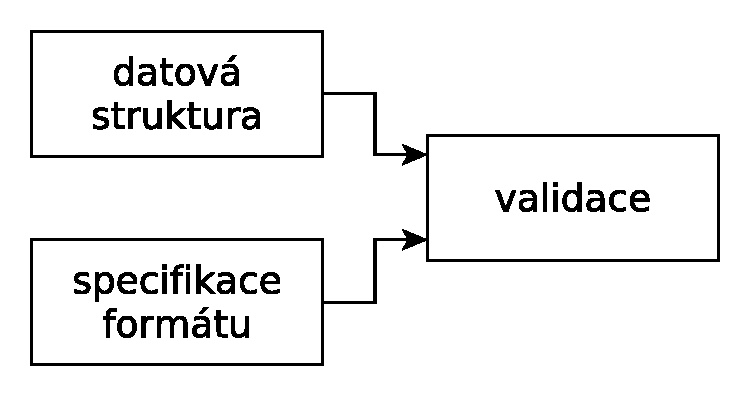
\includegraphics[width=1.4\textwidth]{../../img/validation_process.pdf}\\
	\end{minipage}
\end{frame}

\begin{frame}
	\frametitle{Validace}
	\vspace{15pt}
	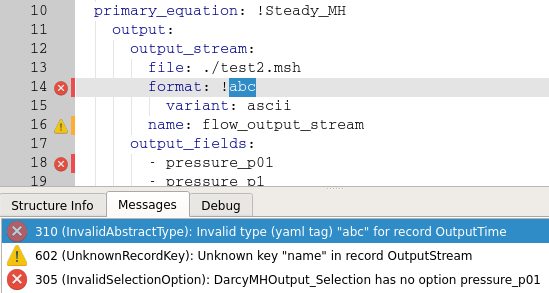
\includegraphics[width=\textwidth]{img/validation.png}
\end{frame}

\begin{frame}[fragile]
	\frametitle{Nápověda a automatické doplňování}
	\vspace*{-20pt}
	\pause
	\begin{minipage}[t]{0.55\textwidth}
	\begin{block}{Nápověda}
	\begin{itemize}[<+>]
		\item kontextová dokumentace
		\item alternativa k~rozsáhlé referenční dokumentaci
	\end{itemize}
	\end{block}
	\begin{block}{Automatické doplňování}
	\begin{itemize}[<+>]
		\item doplňuje názvy klíčů, hodnoty výčtového typu, datové typy abstraktních záznamů
		\item citlivé na kontext
		\item filtrování v~průběhu psaní
	\end{itemize}
	\end{block}
	\end{minipage}
	\hspace*{-10pt}
	\begin{minipage}[t]{0.35\textwidth}
	\vspace{45pt}
	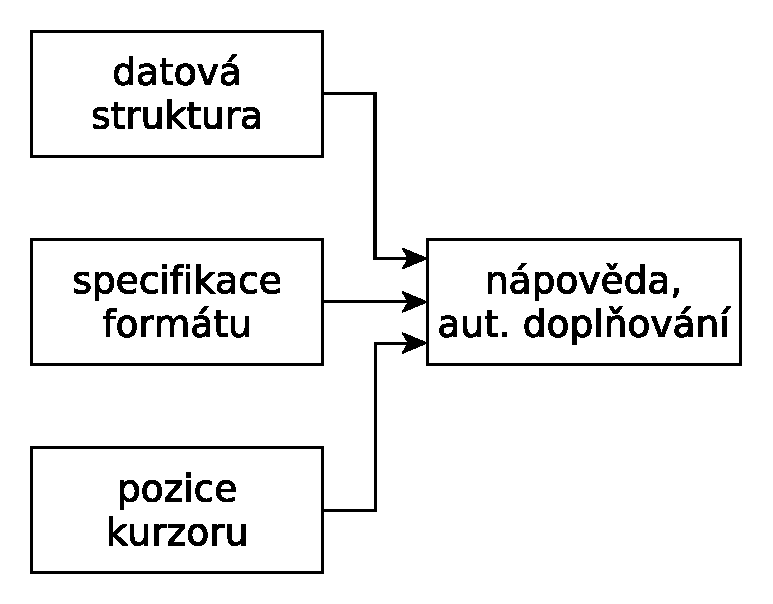
\includegraphics[width=1.4\textwidth]{../../img/documentation_autocompletion.pdf}\\
	\end{minipage}
\end{frame}
\begin{frame}
	\frametitle{Kontextová nápověda}
	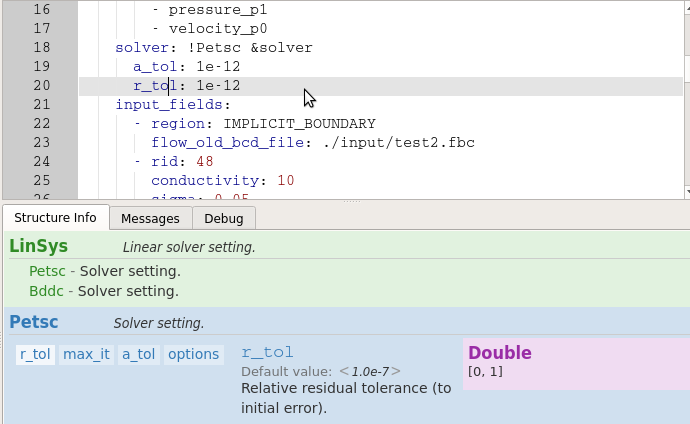
\includegraphics[width=\textwidth]{img/doc_solver.png}
\end{frame}

\begin{frame}
	\frametitle{Kontextová nápověda}
	\vspace{10pt}
	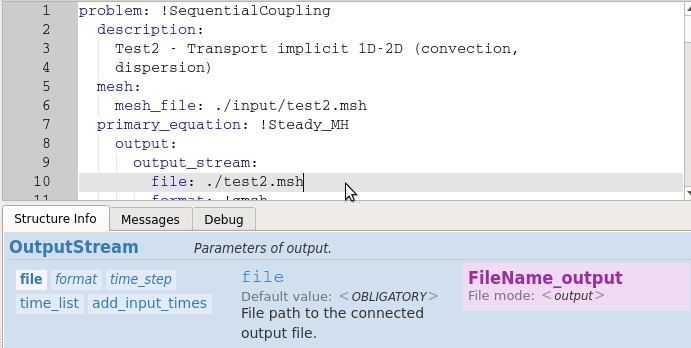
\includegraphics[width=\textwidth]{img/doc_file.png}
\end{frame}

\begin{frame}
	\frametitle{Automatické doplňování}
	\hspace{65pt}
	\vspace{0pt}
	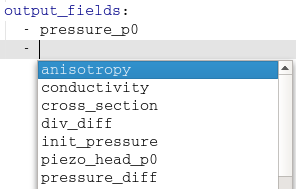
\includegraphics[width=0.45\textwidth]{img/autocompletion_all.png}\\
	\vspace*{15pt}
	\hspace{65pt}
	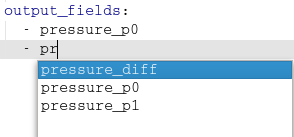
\includegraphics[width=0.45\textwidth]{img/autocompletion_filtered.png}\\
\end{frame}


\begin{frame}
	\frametitle{Shrnutí}
	\vspace{-5pt}
	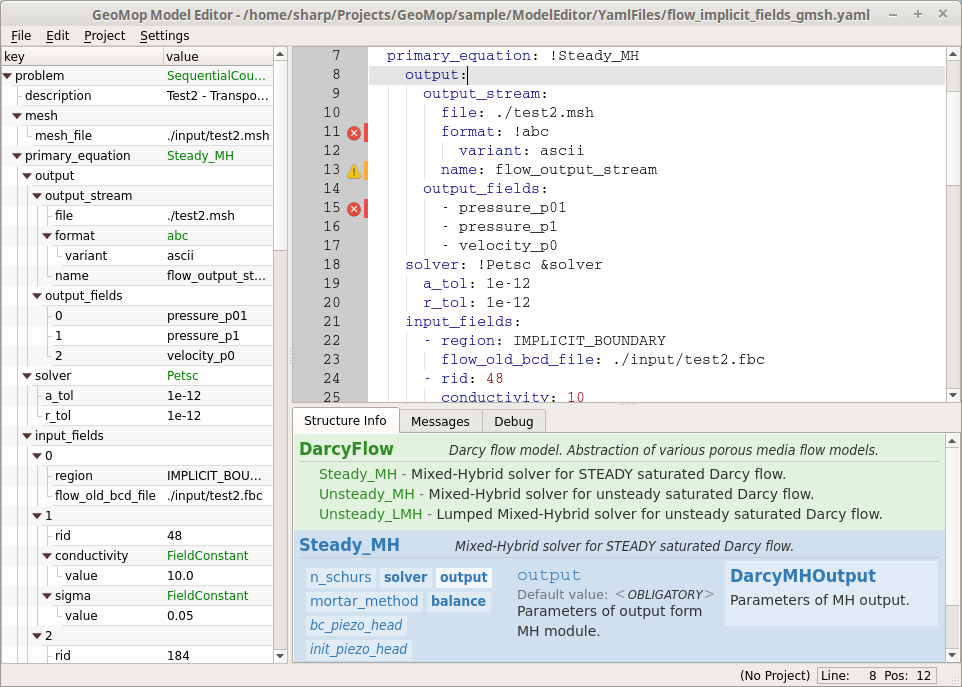
\includegraphics[width=0.9\textwidth]{img/gui.png}\\
\end{frame}

\begin{frame}{}{}
\begin{center}
\huge Děkuji za pozornost.
\end{center}
\end{frame}


\end{document}
